\documentclass[12pt,letterpaper]{article}
\usepackage{graphicx,textcomp}
\usepackage{natbib}
\usepackage{setspace}
\usepackage{fullpage}
\usepackage{color}
\usepackage[reqno]{amsmath}
\usepackage{amsthm}
\usepackage{fancyvrb}
\usepackage{amssymb,enumerate}
\usepackage[all]{xy}
\usepackage{endnotes}
\usepackage{lscape}
\newtheorem{com}{Comment}
\usepackage{float}
\usepackage{hyperref}
\newtheorem{lem} {Lemma}
\newtheorem{prop}{Proposition}
\newtheorem{thm}{Theorem}
\newtheorem{defn}{Definition}
\newtheorem{cor}{Corollary}
\newtheorem{obs}{Observation}
\usepackage[compact]{titlesec}
\usepackage{dcolumn}
\usepackage{tikz}
\usetikzlibrary{arrows}
\usepackage{multirow}
\usepackage{xcolor}
\newcolumntype{.}{D{.}{.}{-1}}
\newcolumntype{d}[1]{D{.}{.}{#1}}
\definecolor{light-gray}{gray}{0.65}
\usepackage{url}
\usepackage{listings}
\usepackage{color}

\definecolor{codegreen}{rgb}{0,0.6,0}
\definecolor{codegray}{rgb}{0.5,0.5,0.5}
\definecolor{codepurple}{rgb}{0.58,0,0.82}
\definecolor{backcolour}{rgb}{0.95,0.95,0.92}

\lstdefinestyle{mystyle}{
	backgroundcolor=\color{backcolour},   
	commentstyle=\color{codegreen},
	keywordstyle=\color{magenta},
	numberstyle=\tiny\color{codegray},
	stringstyle=\color{codepurple},
	basicstyle=\footnotesize,
	breakatwhitespace=false,         
	breaklines=true,                 
	captionpos=b,                    
	keepspaces=true,                 
	numbers=left,                    
	numbersep=5pt,                  
	showspaces=false,                
	showstringspaces=false,
	showtabs=false,                  
	tabsize=2
}
\lstset{style=mystyle}
\newcommand{\Sref}[1]{Section~\ref{#1}}
\newtheorem{hyp}{Hypothesis}

\title{Problem Set 2/}
\date{Jia Lyu/ 23370062}
\author{Quant Methods 1/Due: October 14, 2024}

\begin{document}
	\maketitle
	\section*{Instructions}
\begin{itemize}
	\item Please show your work! You may lose points by simply writing in the answer. If the problem requires you to execute commands in \texttt{R}, please include the code you used to get your answers. Please also include the \texttt{.R} file that contains your code. If you are not sure if work needs to be shown for a particular problem, please ask.
	\item Your homework should be submitted electronically on GitHub.
	\item This problem set is due before 23:59 on Monday October 14, 2024. No late assignments will be accepted.

\end{itemize}

	
	\vspace{.5cm}
	\section*{Question 1: Political Science}
		\vspace{.25cm}
	The following table was created using the data from a study run in a major Latin American city.\footnote{Fried, Lagunes, and Venkataramani (2010). ``Corruption and Inequality at the Crossroad: A Multimethod Study of Bribery and Discrimination in Latin America. \textit{Latin American Research Review}. 45 (1): 76-97.} As part of the experimental treatment in the study, one employee of the research team was chosen to make illegal left turns across traffic to draw the attention of the police officers on shift. Two employee drivers were upper class, two were lower class drivers, and the identity of the driver was randomly assigned per encounter. The researchers were interested in whether officers were more or less likely to solicit a bribe from drivers depending on their class (officers use phrases like, ``We can solve this the easy way'' to draw a bribe). The table below shows the resulting data.

\newpage
\begin{table}[h!]
	\centering
	\begin{tabular}{l | c c c }
		& Not Stopped & Bribe requested & Stopped/given warning \\
		\\[-1.8ex] 
		\hline \\[-1.8ex]
		Upper class & 14 & 6 & 7 \\
		Lower class & 7 & 7 & 1 \\
		\hline
	\end{tabular}
\end{table}

\begin{enumerate}
	
	\item [(a)]
	Calculate the $\chi^2$ test statistic by hand/manually (even better if you can do "by hand" in \texttt{R}).\\
	\lstinputlisting[language=R, firstline=3, lastline=32]{PS02.J.L.R} 
	\item [(b)]
	Now calculate the p-value from the test statistic you just created (in \texttt{R}).\footnote{Remember frequency should be $>$ 5 for all cells, but let's calculate the p-value here anyway.}  What do you conclude if $\alpha = 0.1$?\\
	\lstinputlisting[language=R, firstline=37, lastline=51]{PS02.J.L.R} 
	The p-value(1.1502282) is greater than alpha(0.1),so we cannot reject the null hypothesis,and there is no significant association between a driver's social class and the police officer's behavior.\\
	
	\item [(c)] Calculate the standardized residuals for each cell and put them in the table below.
	\lstinputlisting[language=R, firstline=62, lastline=79]{PS02.J.L.R} 
	
	\begin{table}[h]
		\centering
		\begin{tabular}{l | c c c }
			& Not Stopped & Bribe requested & Stopped/given warning \\
			\\[-1.8ex] 
			\hline \\[-1.8ex]
			Upper class  &0.3220306  &-1.516426  &1.649103  \\
			\\
			Lower class  &-0.2740361  &1.929528   & -1.523026  \\
			
		\end{tabular}
	\end{table}
	
	
	\vspace{7cm}
	\item [(d)] How might the standardized residuals help you interpret the results?  
	\\   The standardized residuals for each cell in the contingency table provide insight into how the observed frequencies compare to the expected frequency of police solicitation based on driver rank.
	
	Upper level observations:
	No stops: The standardized residual is 0.3220306, which is positive and close to zero. This indicates that the observed number of upper class drivers not stopped is slightly higher than expected, but the deviation is small and not statistically significant.
	Solicited Bribes: The standardized residual is -1.516426, which is negative and relatively large in absolute value (greater than 1). This indicates that the observed number of upper class drivers being solicited for bribes is significantly lower than expected, suggesting that they are less likely to be solicited for bribes than the model predicts.
	Stopped/Warned: The standardized residual of 1.649103 is positive and greater than 1. This indicates that the observed number of upper class drivers stopped or warned is significantly higher than expected, suggesting that they are more likely to be stopped compared to predictions.
	
	Lower Class Observations:
	Not Stopped: The standardized residual of -0.2740361 is negative and close to zero. This suggests that drivers in the lower strata are slightly less likely than expected to not be stopped, but this deviation is small and not statistically significant.
	Soliciting Bribes: The standardized residual is 1.929528, which is positive and relatively large (greater than 1). This suggests that lower-class drivers are solicited for bribes more frequently than expected, indicating a possible bias against them.
	Stop/Warning: The standardized residual is -1.523026, which is negative and significant (absolute value greater than 1). This indicates that lower tier drivers were stopped or warned less frequently than expected, suggesting that they may have been treated differently than upper tier drivers.
	
	Conclusion:
	The standardized residual values for both the upper and lower strata are within the range of [-2, 2], indicating that there are no extreme deviations from what would be expected under the null hypothesis. Although there were significant differences in the way the strata interacted with police officers regarding bribery and stops, these differences do not reflect significant anomalies in the data.
	In summary, the standardized residuals provide insight into possible bias or discrimination in police behavior based on driver class, helping to inform discussions about corruption and inequality in law enforcement practices.
	

	
\end{enumerate}
\newpage

\section*{Question 2: Economics}
Chattopadhyay and Duflo were interested in whether women promote different policies than men.\footnote{Chattopadhyay and Duflo. (2004). ``Women as Policy Makers: Evidence from a Randomized Policy Experiment in India. \textit{Econometrica}. 72 (5), 1409-1443.} Answering this question with observational data is pretty difficult due to potential confounding problems (e.g. the districts that choose female politicians are likely to systematically differ in other aspects too). Hence, they exploit a randomized policy experiment in India, where since the mid-1990s, $\frac{1}{3}$ of village council heads have been randomly reserved for women. A subset of the data from West Bengal can be found at the following link: \url{https://raw.githubusercontent.com/kosukeimai/qss/master/PREDICTION/women.csv}\\

\noindent Each observation in the data set represents a village and there are two villages associated with one GP (i.e. a level of government is called "GP"). Figure~\ref{fig:women_desc} below shows the names and descriptions of the variables in the dataset. The authors hypothesize that female politicians are more likely to support policies female voters want. Researchers found that more women complain about the quality of drinking water than men. You need to estimate the effect of the reservation policy on the number of new or repaired drinking water facilities in the villages.
\vspace{.5cm}
\begin{figure}[h!]
	\caption{\footnotesize{Names and description of variables from Chattopadhyay and Duflo (2004).}}
	\vspace{.5cm}
	\centering
	\label{fig:women_desc}
	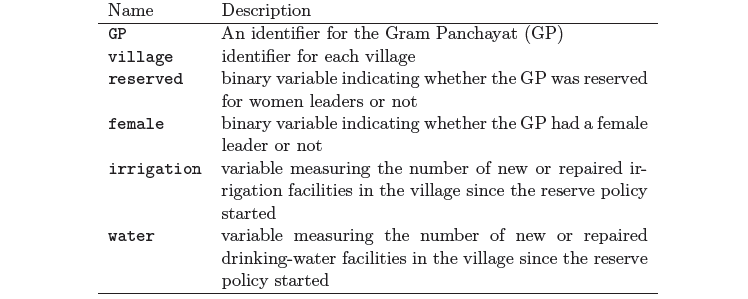
\includegraphics[width=1.1\textwidth]{women_desc.png}
\end{figure}		

\newpage
\begin{enumerate}
	\item [(a)] State a null and alternative (two-tailed) hypothesis. 
	
	Null Hypothesis (H0): There is no difference in the number of new or repaired drinking water facilities between villages with reserved and unreserved council heads.\\

	Alternative Hypothesis (Ha): There is a difference in the number of new or repaired drinking water facilities between villages with reserved and unreserved council heads.\\
	
	
	\item [(b)] Run a bivariate regression to test this hypothesis in \texttt{R} (include your code!).
	\lstinputlisting[language=R, firstline=96, lastline=108]{PS02.J.L.R} 
	
	\begin{figure}[h!]\centering
		\caption{\footnotesize{results}}
		\label{fig:9}
		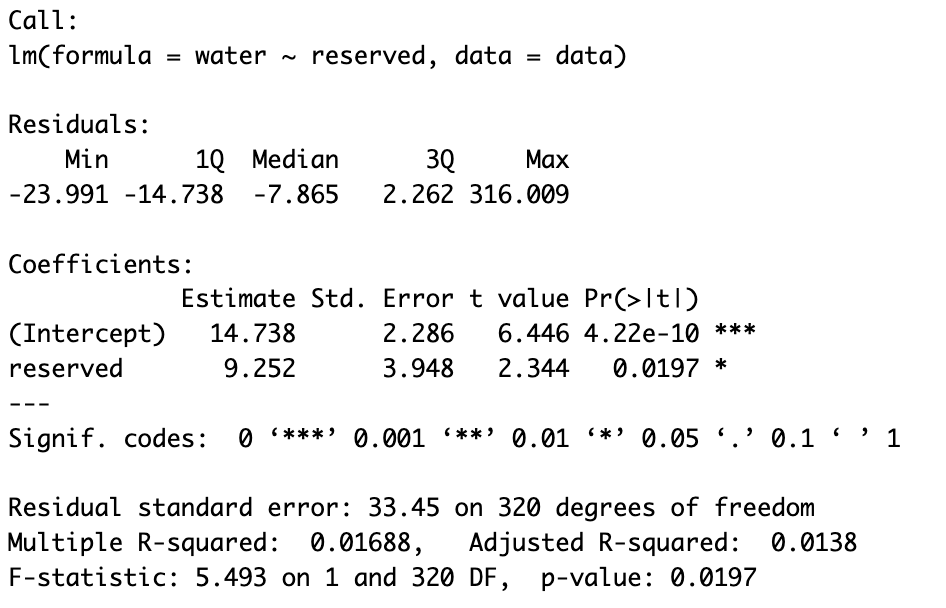
\includegraphics[width=.75\textwidth]{question2.b.png}
	\end{figure}
	\newpage
	\item [(c)] Interpret the coefficient estimate for reservation policy. 
	
	The coefficient estimate Std.for the reservation policy is 9.252,meaning that 
	there is a positive association between the reservation policy and the number of new or repaired drinking water facilities in villages. 
	On average, villages that implemented the reservation policy had 9.252 more such facilities compared to those without the policy.\\
	
\end{enumerate}

\end{document}
